\documentclass{standalone}
\usepackage{tikz}
\begin{document}
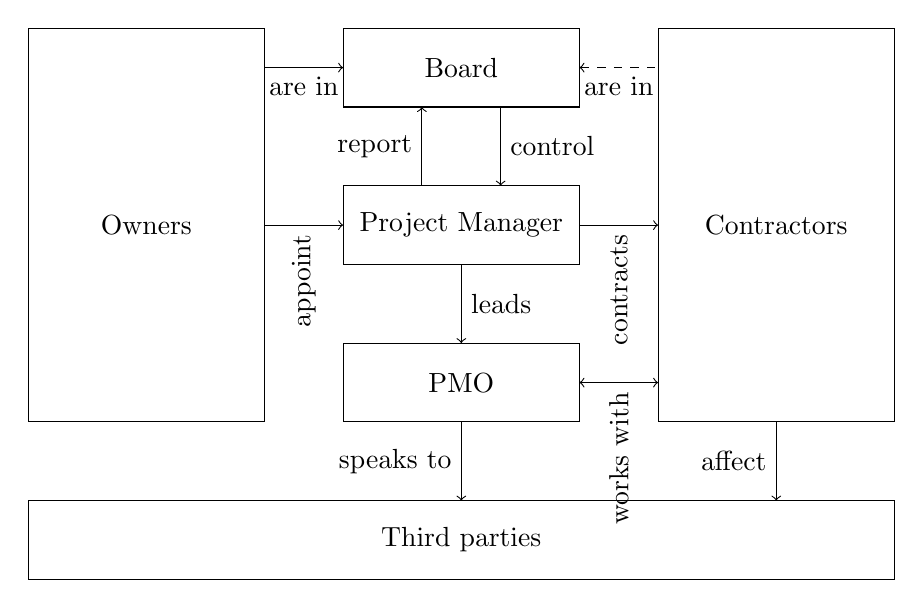
\begin{tikzpicture}
    \draw (-5,0) rectangle node {Third parties} (6,1);
    \draw (-5,2) rectangle node {Owners} (-2,7);
    \draw (-1,6) rectangle node {Board} (2,7);
    \draw (-1,4) rectangle node {Project Manager} (2,5);
    \draw (-1,2) rectangle node {PMO} (2,3);
    \draw (3,2) rectangle node {Contractors} (6,7);
    \draw[->] (-2,6.5) -- node[below] {are in} (-1,6.5);
    \draw[<-,dashed] (2,6.5) -- node[below] {are in} (3,6.5);
    \draw[<-] (0,6) --  node[left] {report} (0,5);
    \draw[->] (1,6) -- node[right] {control} (1,5);
    \draw[->] (-2,4.5) -- node[left, rotate=90] {appoint} (-1,4.5);
    \draw[->] (0.5,4) -- node[right] {leads} (0.5,3);
    \draw[->] (0.5,2) -- node[left] {speaks to} (0.5,1);
    \draw[<-] (3,4.5) -- node[left, rotate=90] {contracts} (2,4.5);
    \draw[<->] (3,2.5) -- node[left, rotate=90] {works with} (2,2.5);
    \draw[->] (4.5,2) -- node[left] {affect}  (4.5,1);
\end{tikzpicture}
\end{document}